\documentclass[xcolor=pdftex,romanian,colorlinks]{beamer}

\usepackage[export]{adjustbox}
\usepackage{../tslides}
\usepackage[all]{xy}
\usepackage{pgfplots}
\usepackage{flowchart}
\usetikzlibrary{arrows,positioning,calc}
\lstset{language=Haskell}
\lstset{escapeinside={(*@}{@*)}}

\AtBeginSection[]{
  \begin{frame}
  \vfill
  \centering
  \begin{beamercolorbox}[sep=8pt,center,shadow=true,rounded=true]{title}
    \usebeamerfont{title}\insertsectionhead\par%
  \end{beamercolorbox}
  \vfill
  \end{frame}
}


\title[PD---Monade]{Programare declarativă\thanks{bazat pe cursul \emph{Informatics 1: Functional Programming} de la \emph{University of Edinburgh}}}

\subtitle{Efecte laterale --- Monade}

\begin{document}
\begin{frame}
  \titlepage
\end{frame}

\section{Monade}

\begin{frame}[fragile]{Monoizi}
Un monoid e o structură algebrică dată de o operație binară \lstinline$(@@)$ și o valoare u, astfel încât \lstinline$(@@)$ este asociativă și are element neutru u.

\begin{asciihs}
   u @@ x              =   x
   x @@ u              =   x
   (x @@ y) @@ z       =   x @@ (y @@ z)
\end{asciihs}
\begin{block}
{Exemple de monoizi}
\begin{itemize}
\item \lstinline$(+)$ și \lstinline$0$
\item \lstinline$(*)$ și \lstinline$1$
\item \lstinline$(||)$ și \lstinline$False$
\item \lstinline$(&&)$ și \lstinline$True$
\item \lstinline$(++)$ și \lstinline$[]$
\item \lstinline$(>>)$ și \lstinline$done$
\end{itemize}
\end{block}
\end{frame}


\begin{frame}[fragile]{Monade}
\lstinline$(>>)$ and \lstinline$done$ verifică axiomele de monoid.
\begin{asciihs}
   done >> m          =   m
   m >> done          =   m
   (m >> n) >> o      =   m >> (n >> o)
\end{asciihs}

\vfill
În mod asemănator, \lstinline$(>>=)$ și \lstinline$return$ verifică axiomele de \structure{monadă}
\begin{asciihs}
  return v >>= \x -> m        =  m[v/x]
  m >>= \x -> return x        =  m
  (m >>= \x -> n) >>= \y-> o  =  m >>= \x -> (n >>= \y -> o)
\end{asciihs}

\onslide<2>
\vfill
Alternativ, folosind ideea de \structure{continuare}:
\begin{asciihs}
  return v >>= k    =  k v
  m >>= return      =  m
  (m >>= k) >>= k'  =  m >>= \x -> (k x >>= k')
\end{asciihs}
\end{frame}

%
%
%Similarly, (>>=) and return satisfy the laws of a monad.
%   return v >>= \x -> m               =   m[x:=v]
%   m >>= \x -> return x               =   m
%   (m >>= \x -> n) >>= \y-> o         =   m >>= \x -> (n >>= \y -> o)
%\begin{frame}[fragile]{}
%\begin{asciihs}
%\end{asciihs}
%\end{frame}

%Laws of Let
%We know that (>>) and done satisfy the laws of a monoid.
%   done >> m           =   m
%   m >> done           =   m
%   (m >> n) >> o       =   m >> (n >> o)
%
%                    =   let x = m in (let y = n in o)
\begin{frame}[fragile]{Monade, notație \lstinline$do$ și \lstinline$let$}
\lstinline$(>>=)$ și \lstinline$return$ verifică axiomele de monadă.
\begin{asciihs}
  return v >>= \x -> m        =  m[v/x]
  m >>= \x -> return x        =  m
  (m >>= \x -> n) >>= \y-> o  =  m >>= \x -> (n >>= \y -> o)
\end{asciihs}

%
%The three monad laws have analogues in “let” notation.
Axiome analoage pentru let:
\begin{asciihs}
   let x = v in m   =   m[v/x]
   let x = m in x   =   m
   let y = (let x = m in n) in o
                    =   let x = m in (let y = n in o)
\end{asciihs}

\onslide<2>
Notație \lstinline$do$ pentru expresiile de mai sus:
\begin{asciihs}
  do {x <- return v ; m}         =  m[v/x] 
  do {x <- m ; return x}         =  m
  do {y <- do {x <- m ; n} ; o}  =  do {x <- m ; 
                                        do {y <- n ; o}}
\end{asciihs}

\end{frame}

\begin{frame}[fragile]{Axiomele lui let și efectele laterale}
\begin{asciihs}
   let x = v in m   =   m[v/x]
   let x = m in x   =   m
   let y = (let x = m in n) in o
                    =   let x = m in (let y = n in o)
\end{asciihs}
Axiomele acestea țin și în limbaje cu efecte laterale dacă v e valoare.

În limbaje „pure” precum Haskell, prima axiomă poate fi întărită astfel:
\begin{asciihs}
   let x = n in m   =   m[n/x]
\end{asciihs}
cu înțelesul că o variabilă poate fi înlocuită peste tot cu orice termen. Deoarece limbajul este pur, evaluarea lui n nu va produce efecte laterale, indiferent de câte ori este evaluat.
\end{frame}
%“Let” in languages with and without effects
%   let x = v in m   =   m[x:=v]
%   let x = m in x   =   m
%   let y = (let x = m in n) in o
%                    =   let x = m in (let y = n in o)
%
%These laws hold even in languages with side effects. For the first law to be true, v
%must be not an arbitrary term but a value, such as a constant or a variable (but not
%a function application). A value immediately evaluates to itself, hence it can have
%no side effects.
%While in such languages one only has the above three laws for “let”, in Haskell
%one has a much stronger law, where one may replace a variable by any term, rather
%than by any value.
%   let x = n in m         =   m[x:=n]


\begin{frame}[fragile]{Clasa de tipuri \lstinline$Monad$}
{Control.Monad.Monad}
\begin{asciihs}
  class Monad m where
    return :: a -> m a
    (>>=) :: m a -> (a -> m b) -> m b
\end{asciihs}
\begin{itemize}
\item m este un constructor de tipuri

m a --- tipul \structure{computațiilor} care produc rezultate de tip a
\item Tipul \lstinline$a -> m b$ este tipul \structure{continuărilor}

Continuare: O funcție care folosește un rezultat de tip a pentru a produce o computatie de tip b

\item \lstinline$(>>=)$ este operația de „secvențiere” a computațiilor

\item \lstinline$return$ este continuarea trivială

Pentru un v dat, produce computația care va avea ca rezultat acel v.
\end{itemize}
\end{frame}

%The Monad type class




%        Part VII
%
%Roll your own monad—IO

\section{Să ne definim propria monadă IO}


\begin{frame}[fragile]{Monada MyIO}{partea I}
\begin{asciihs}
   module MyIO(MyIO, myPutChar, myGetChar, convert) where

   type Input = String
   type Remainder = String
   type Output = String

   newtype MyIO a  =  MyIO (Input -> (a, Remainder, Output))

   apply :: MyIO a -> Input -> (a, Remainder, Output)
   apply (MyIO f) inp = f inp
\end{asciihs}

\begin{block}{Observație: Tipul MyIO is abstract}
\begin{itemize} 
\item Sunt exportate doar tipul MyIO, myPutChar, myGetChar, convert 

(și operațiile de monadă)
\item Nu este exportat constructorul MyIO și nici operația apply
\end{itemize}
\end{block} 
\end{frame}

%My own IO monad (1)
%


\begin{frame}[fragile]{Monada MyIO}{partea II}
\begin{asciihs}
 myPutChar :: Char -> MyIO ()
 myPutChar c = MyIO (\ inp -> ((), inp, [c]))

 myGetChar :: MyIO Char
 myGetChar = MyIO (\ (ch:remainder) -> (ch, remainder, ""))
\end{asciihs}

\begin{block}
{Exemplu}
\begin{asciihs}
   apply myGetChar "abc" == ('a',    "bc", "")
   apply myGetChar "bc"   == ('b',   "c", "")
   apply (myPutChar 'A') "def" ==    ((), "def", "A")
   apply (myPutChar 'B') "def" ==    ((), "def", "B")
\end{asciihs}
\end{block}

\end{frame}



\begin{frame}[fragile]{Monada MyIO}{partea III}
\begin{asciihs}
   instance Monad MyIO where
     return x = MyIO (\ inp -> (x, inp, ""))
     m >>= k  = MyIO (\ inp ->
                    let (x, rem1, out1) = apply m inp
                        (y, rem2, out2) = apply (k x) rem1 
                      in
                        (y, rem2, out1++out2))
\end{asciihs}

\begin{block}
{Exemplu}
\vspace{-2ex}
\begin{asciihs}
   apply
     (myGetChar >>= \x -> myGetChar >>= \y -> return [x,y])
     "abc"
   == ("ab", "c", "")
   apply (myPutChar 'A' >> myPutChar 'B') "def"
   == ((), "def", "AB")
   apply (myGetChar >>= \x -> myPutChar (toUpper x)) "abc"
   == ((), "bc", "A")
\end{asciihs}
\end{block}

\end{frame}


%My own IO monad (3)
%
%For example

\begin{frame}[fragile]{Monada MyIO}{partea IV}
\begin{asciihs}
   convert :: MyIO () -> IO ()
   convert m = interact (\inp ->
                   let (x, rem, out) = apply m inp in
                   out)
\end{asciihs}

Unde
\begin{asciihs}
   interact :: (String -> String) -> IO ()
\end{asciihs}
face parte din biblioteca standard, si face următoarele:
\begin{itemize}
\item Citește stream-ul de intrare la un șir de caractere (leneș)
\item Aplică funcția dată ca parametru acestui șir
\item Trimite șirul rezultat către stream-ul de ieșire (tot leneș)
\end{itemize}
\end{frame}


%My own IO monad (4)
%   convert :: MyIO () -> IO ()
%   convert m = interact (\inp ->
%                   let (x, rem, out) = apply m inp in
%                   out)
%
%Here
%   interact :: (String -> String) -> IO ()
%
%is part of the standard prelude. The entire input is converted to a string (lazily) and
%passed to the function, and the result from the function is printed as output (also
%lazily).


\begin{frame}[fragile]{Folosirea monadei MyIO}
{partea I}
\begin{asciihs}
  module MyEcho where

  import Char
  import MyIO

  myPutStr :: String -> MyIO ()
  myPutStr = foldr (>>) (return ()) . map myPutChar

  myPutStrLn :: String -> MyIO ()
  myPutStrLn s = myPutStr s >> myPutChar '\n'
\end{asciihs}
\end{frame}


%Using my own IO monad (1)

\begin{frame}[fragile]{Folosirea monadei MyIO}
{partea II}
\vspace{-2ex}
\begin{asciihs}
  myGetLine :: MyIO String
  myGetLine = myGetChar >>= \x ->
               if x == '\n' then
                 return []
               else
                 myGetLine >>= \xs ->
                 return (x:xs)

  myEcho :: MyIO ()
  myEcho = myGetLine >>= \line ->
            if line == "" then
              return ()
            else
              myPutStrLn (map toUpper line) >>
              myEcho

  main :: IO ()
  main = convert myEcho
\end{asciihs}
\end{frame}


%Using my own IO monad (2)

\begin{frame}[fragile]{În execuție}
{partea I}
\begin{asciihs}
  10-monade$ runghc MyEcho
  This is a test.
  THIS IS A TEST.
  It is only a test.
  IT IS ONLY A TEST.
  Were this a real emergency, you'd be dead now.
  WERE THIS A REAL EMERGENCY, YOU'D BE DEAD NOW.

  10-monade$
\end{asciihs}
\end{frame}

\begin{frame}[fragile]{Folosind notația \lstinline$do$}
\vspace{-2ex}
\begin{asciihs}
  myGetLine :: MyIO String
  myGetLine = do {
                 x <- myGetChar;
                 if x == '\n' then
                   return []
                 else do {
                   xs <- myGetLine;
                   return (x:xs)
                 }
               }
  myEcho :: MyIO ()
  myEcho = do {
              line <- myGetLine;
              if line == "" then
                return ()
              else do {
                myPutStrLn (map toUpper line);
                myEcho
              } }
\end{asciihs}
\end{frame}


%You can use “do” notation, too
%     Part VIII
%
%The monad of lists
\section{Monada listelor}

\begin{frame}[fragile]{Monada listelor}
Definiția în biblioteca standard:
\begin{asciihs}
     class Monad m where
       return :: a -> m a
       (>>=) :: m a -> (a -> m b) -> m b

     instance Monad [] where

       return       :: a -> [a]
       return x     = [ x ]

       (>>=)        :: [a] -> (a -> [b]) -> [b]
       m >>= k      = [ y | x <- m, y <- k x ]
\end{asciihs}
Recursiv:
\vspace{-1ex}
\begin{asciihs}
       [] >>= k            =   []
       (x:xs) >>= k        =   (k x) ++ (xs >>= k)
\end{asciihs}
Cu funcții de ordin înalt:
\vspace{-1ex}
\begin{asciihs}
       m >>= k    =   concat (map k m)
\end{asciihs}
\end{frame}

\begin{frame}[fragile]{Monada listelor}{Intuiție}
\begin{asciihs}
     instance Monad [] where

       return       :: a -> [a]
       return x     = [ x ]

       (>>=)        :: [a] -> (a -> [b]) -> [b]
       m >>= k      = [ y | x <- m, y <- k x ]
\end{asciihs}
\begin{itemize}
\item Tipul [a] tipul computațiilor nedetermniste, 

care pot întoarce 0, 1, sau mai multe rezultate
\vitem \lstinline$return$ este continuare care dat fiind un rezultat, întoarce
(determinst) doar acel rezultat
\vitem \lstinline$m >>= k$ aplică continuarea $k$ fiecărui rezultat al lui x
și agreghează rezultatele
\end{itemize}
\end{frame}




%The monad of lists


\begin{frame}[fragile]{Descrieri de liste și monada listelor}
{Notație \lstinline$do$}
\begin{asciihs}
   pairs :: Int -> [(Int, Int)]
   pairs n = [ (i,j) | i <- [1..n], j <- [(i+1)..n] ]
\end{asciihs}
este echivalentă cu
\begin{asciihs}
   pairs' :: Int -> [(Int, Int)]
   pairs' n = do {
                  i <- [1..n];
                  j <- [(i+1)..n];
                  return (i,j)
                }
\end{asciihs}
Exemplu:
\begin{asciihs}
   *Main> pairs 4
   [(1,2),(1,3),(1,4),(2,3),(2,4),(3,4)]
   *Main> pairs' 4
   [(1,2),(1,3),(1,4),(2,3),(2,4),(3,4)]
\end{asciihs}
\end{frame}


\begin{frame}[fragile]{Monade cu structură de monoid}
\vspace{-1ex}
Definiția în biblioteca standard:
\begin{asciihs}
   class Monad m => MonadPlus m where
     mzero :: m a
     mplus :: m a -> m a -> m a

   instance MonadPlus [] where
      mzero     :: [a]
      mzero     = []

      mplus     :: [a] -> [a] -> [a]
      mplus     = (++)

   guard :: MonadPlus m => Bool -> m ()
   guard False = mzero
   guard True   = return ()

   msum :: MonadPlus m => [m a] -> m a
   msum = foldr mplus mzero
\end{asciihs}
\end{frame}


%Monads with plus
%In the standard prelude:

\begin{frame}[fragile]{Descrieri de liste cu filtrare}
\begin{asciihs}
   pairs'' :: Int -> [(Int, Int)]
   pairs'' n = [ (i,j) | i <- [1..n], j <- [1..n], i < j ]
\end{asciihs}
este echivalentă cu
\begin{asciihs}
   pairs''' :: Int -> [(Int, Int)]
   pairs''' n = do {
                    i <- [1..n];
                    j <- [1..n];
                    guard (i < j);
                    return (i,j)
                  }
\end{asciihs}
Exemplu
\begin{asciihs}
   *Main> pairs'' 4
   [(1,2),(1,3),(1,4),(2,3),(2,4),(3,4)]
   *Main> pairs''' 4
   [(1,2),(1,3),(1,4),(2,3),(2,4),(3,4)]
\end{asciihs}
\end{frame}

\section{Analiză sintactică}

\begin{frame}[fragile]{Tipul unui analizor sintactic}
\begin{block}
{Prima încercare}
\begin{asciihs}
   type Parser a = String -> a
\end{asciihs}
\onslide<2->
\begin{itemize}
\item Dar cel puțin pentru rezultate parțiale, va mai rămâne ceva de analizat
\end{itemize}
\end{block}
%
%Second attempt:
\onslide<3->
\begin{block}
{A doua încercare}
\begin{asciihs}
   type Parser a = String -> (a, String)
\end{asciihs}
\onslide<4>
\begin{itemize}
\item Dar dacă gramatica e ambiguă?
\item Dar dacă intrarea nu corespunde nici unui element din a?
\end{itemize}
\end{block}
\end{frame}


%Parser type
%
%
%
%                         A parser for things
%                     is a function from strings
%                           to lists of pairs
%                        Of things and strings
%                                             —Graham Hutton
\begin{frame}[fragile]{Tipul unui analizor sintactic}{A treia încercare}
\hfill \href{http://www.willamette.edu/~fruehr/haskell/seuss.html}{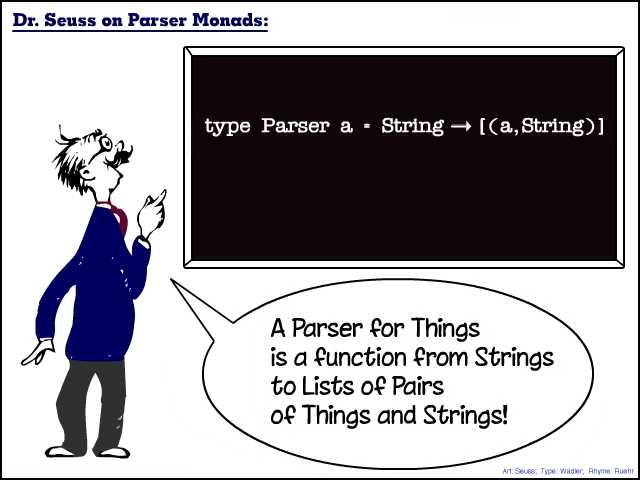
\includegraphics[scale=.4]{SeussFinal2}}\hfill\;
\end{frame}

\begin{frame}[fragile]{Modulul Parser}
{partea I}
\begin{asciihs}
  module Parser(Parser,apply,parse,char,spot,token,
    star,plus,parseInt) where

  import Char
  import Monad

  -- Tipul (incapsulat) Parser
  newtype Parser a = Parser (String -> [(a, String)])

  -- Folosirea unui parser (functie privata)
  apply :: Parser a -> String -> [(a, String)]
  apply (Parser f) s = f s

  -- Daca exista parsare, da prima varianta
  parse :: Parser a -> String -> a
  parse m s = head [ x | (x,t) <- apply m s, t == "" ]
\end{asciihs}
\end{frame}


%Module Parser

\begin{frame}[fragile]{Modulul Parser}{partea II: Parser e monadă}
\begin{asciihs}

  --   class Monad m where
  --     return :: a -> m a
  --     (>>=) :: m a -> (a -> m b) -> m b

  instance Monad Parser where
    return x  = Parser (\s -> [(x,s)])
    m >>= k   = Parser (\s ->
                   [ (y, u) |
                     (x, t) <- apply m s,
                     (y, u) <- apply (k x) t ])
\end{asciihs}
\end{frame}


%Parser is a Monad

\begin{frame}[fragile]{Modulul Parser}{partea II: Parser e monadă cu plus}
\begin{asciihs}
  --   class MonadPlus m where
  --     mzero :: m a
  --     mplus :: m a -> m a -> m a

  instance MonadPlus Parser where
    mzero      = Parser (\s -> [])
    mplus m n  = Parser (\s -> apply m s ++ apply n s)
\end{asciihs}

\begin{itemize}
\item mzero reprezintă analizorul sintactic care eșuează tot timpul
\item mplus reprezintă combinarea alternativelor
\end{itemize}

\end{frame}


%Parser is a Monad with Plus
%  -- Some monads have additional structure
%

\begin{frame}[fragile]{Parsare pentru caractere}
\begin{asciihs}
  -- Recunoasterea unui caracter
  char :: Parser Char
  char = Parser f
    where
    f []     = []
    f (c:s) = [(c,s)]

  -- Recunoasterea unui caracter cu o proprietate
  spot :: (Char -> Bool) -> Parser Char
  spot p = Parser f
    where
    f []                 = []
    f (c:s) | p c        = [(c, s)]
            | otherwise = []

  -- Recunoasterea unui anumit caracter
  token :: Char -> Parser Char
  token c = spot (== c)
\end{asciihs}
\end{frame}


%Parsing characters


\begin{frame}[fragile]{Recunoașterea unui caracter cu o proprietate}
{Gărzi și notație \lstinline$do$}
\begin{asciihs}
  spot :: (Char -> Bool) -> Parser Char
  spot p = Parser f
    where
    f []                 = []
    f (c:s) | p c        = [(c, s)]
            | otherwise = []
\end{asciihs}
e echivalentă cu
\begin{asciihs}
  spot :: (Char -> Bool) -> Parser Char
  spot p = do { c <- char; guard (p c); return c }
\end{asciihs}
\end{frame}

\begin{frame}[fragile]{Recunoașterea unui cuvânt cheie}
\begin{asciihs}
  match :: String -> Parser String
  match []      = return []
  match (x:xs) = do
                     y <- token x;
                     ys <- match xs;
                     return (y:ys)
\end{asciihs}
\end{frame}


%Parsing a string

\begin{frame}[fragile]{Recunoașterea unei secvențe repetitive}
\begin{asciihs}
  -- Steluta Kleene (zero, una sau mai multe repetitii)
  star :: Parser a -> Parser [a]
  star p = plus p `mplus` return []

  -- cel putin o repetitie
  plus :: Parser a -> Parser [a]
  plus p = do { x <- p;
                xs <- star p;
                return (x:xs) }
\end{asciihs}
\end{frame}


%Parsing a sequence

\begin{frame}[fragile]{Recunoașterea unui numar întreg}
\begin{asciihs}
  -- Recunoasterea unui numar natural
  parseNat :: Parser Int
  parseNat = do { s <- plus (spot isDigit);
                  return (read s) }

  -- Recunoasterea unui numar negativ
  parseNeg :: Parser Int
  parseNeg = do { token '-';
                  n <- parseNat
                  return (-n) }

  -- Recunoasterea unui numar intreg
  parseInt :: Parser Int
  parseInt = parseNat `mplus` parseNeg
\end{asciihs}
\end{frame}


%Parsing an integer

\begin{frame}[fragile]{Modulul Exp}
\begin{asciihs}
  module Exp where

  import Monad
  import Parser

  data Exp = Lit Int
           | Exp :+: Exp
           | Exp :*: Exp
           deriving (Eq,Show)

  evalExp   :: Exp -> Int
  evalExp   (Lit n)    = n
  evalExp   (e :+: f) = evalExp e + evalExp f
  evalExp   (e :*: f) = evalExp e * evalExp f
\end{asciihs}
\end{frame}


%Module Exp


\begin{frame}[fragile]{Recunoașterea unei expresii}
\begin{asciihs}
  parseExp :: Parser Exp
  parseExp = parseLit `mplus` parseAdd `mplus` parseMul
    where
    parseLit = do { n <- parseInt;
                    return (Lit n) }
    parseAdd = do { token '(';
                    d <- parseExp;
                    token '+';
                    e <- parseExp;
                    token ')';
                    return (d :+: e) }
    parseMul = do { token '(';
                    d <- parseExp;
                    token '*';
                    e <- parseExp;
                    token ')';
                    return (d :*: e) }
\end{asciihs}
\end{frame}


%Parsing an expression

\begin{frame}[fragile]{Recunoașterea unei expresii}{Test}
\begin{asciihs}
  *Exp> parse parseExp "(1+(2*3))"
  Lit 1 :+: (Lit 2 :*: Lit 3)
  *Exp> evalExp (parse parseExp "(1+(2*3))")
  7
  *Exp> parse parseExp "((1+2)*3)"
  (Lit 1 :+: Lit 2) :*: Lit 3
  *Exp> evalExp (parse parseExp "((1+2)*3)")
  9
\end{asciihs}
\end{frame}



\end{document}



